\documentclass[12pt,a4paper]{article}
\usepackage{hyperref}
\usepackage{amsmath}
\usepackage{graphicx}
\usepackage{float}
\usepackage{subfig}
\title{Laboratory 4: Jamming Resistant Communication}
\author{Vasileios Dimitrakis and Niclas Scheuing}
\newtheorem{hypo}{Hypothesis}
\begin{document}
\maketitle

\section{Introduction}

Communication jamming is a technique that entirely prevents or reduces the ability of communicating parties to pass information by the deliberate use of electromagnetic signals. We distinguish the jamming from interference. Devices that simply cause interference are regulated under different regulations.
The jamming is categorized in the intentional and unintentional jamming. The first one occurs when a device transmits in a busy medium without first checking if it is already in use. The second case aims at radio signals, in order to interrupt the communication and prevent availability.
Jamming attack is effective, when the attacker has enough power to transmit, so that the receiver will not be able to receive the message or the jamming signal has certain characteristics that prevent the processor from extracting the original message.

\section{Materials and Methods}
Throughout the lab exercise 4 we used different materials and methods, that are presented below:
\begin{itemize}
\item \emph{SDR - Software Defined Radio}: Is a hardware device that is capable of synthesizing arbitary radio signals.
\item \emph{hostapd}: Is a user space deamon for Access point and authentication servers.
\item \emph{GNU Radio}: Is a free software development toolkit that provides signal processing blocks to implement software-defined radios and signal processing systems. 
\end{itemize}

\section{Terminology and Topology}
In the current lab exercise we examine the following topology and we use the appropriate terminology:
\begin{itemize}
\item \emph{Access Point (AP)}: One machine serves as an Access Point and is used for the communication with the client.
\item \emph{Client (C)}: One PC of the group serves as the client, which sends the ICMP messages through the ping command to AP.
\item \emph{Attacking device}: The attacking machine uses the USRP device to transmit the jamming signal, in order to interrupt the communication.
\item \emph{Monitoring device}: The monitoring device uses the other USRP device to constantly monitor the wireless channel.
\end{itemize}



\section{Setup}
	\subsubsection{Attacking Team}
		In the attacker's configuration, we set a low-pass filter, because this kind of filter removes the noise that is produced by the Noise source outside the band that we observe. Moreover, the low-pass filter determines the bandwidth that the jamming signal will have.
		See \autoref{topo:jam} for the \emph{GNURadio} configuration.
		\begin{figure}
			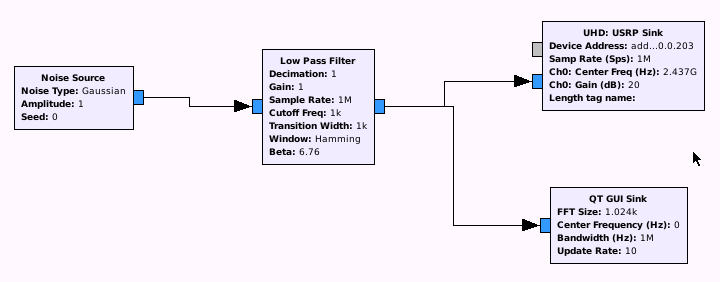
\includegraphics[width=\textwidth]{images/topo1.png}
			\caption{\emph{GNURadio} configuration of the jammer.}
			\label{topo:jam}
		\end{figure}
		
	
	\subsubsection{Monitoring Team}
		The other USRP is used to observe the signals. Its \emph{GNURadio} configuration does nothing but monitoring and can be seen in \autoref{topo:mon}
		
		\begin{figure}
			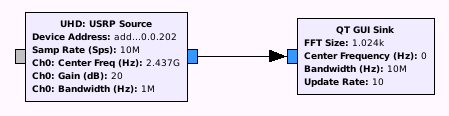
\includegraphics[width=\textwidth]{images/model_mon.png}
			\caption{\emph{GNURadio} configuration of the monitor.}
			\label{topo:mon}
		\end{figure}
	
	\subsection{Channel selection}
		The center frequencies of channels 1, 6 and 11 are $2.412 GHz$, $2.437 GHz$ and $2.462 GHz$, respectively. Every 802.11 Wi-Fi channel has bandwidth equal to $22 MHz$. In this lab exercise, we used for communication the Wi-Fi channels 1, 6 and 11, because they are the only non-overlapping channels and we avoid interference between the experiments of the lab teams.

\section{Experiment}
The Attacking team aims at the interruption of the communication between the client and the Access Point. The characteristics of the jamming signal are configured by the GNU radio software tool and it is transmitted through the USRD2 Software Defined Radio. 

\subsection{Jamming with 1kHz bandwidth}

	The first attempt to jamming the channel was using a Gaussian-random-noise signal with a bandwidth of $1$kHz and a gain of 20dB.
	\begin{hypo}
		The bandwidth of the jamming signal in this case is $1kHz$, which is a very narrow signal. Therefore, we expect that this jamming attack will not significantly affect the transmitting signal and it will not interrupt the communication between the client and the Access Point, which communicate through the ping messages.
	\end{hypo}

	After starting the jamming signal, we can observe that its bandwidth is equal to $1kHz$. Refer to \autoref{1khz:attacker}
	\begin{figure}
		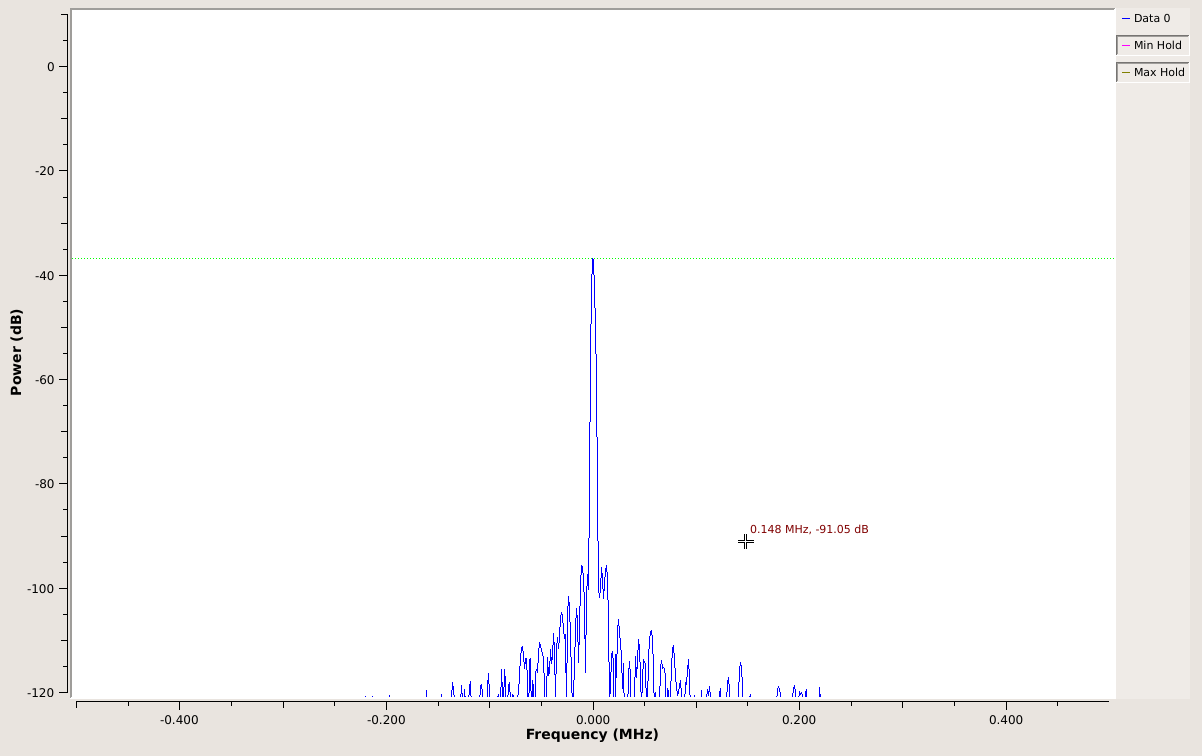
\includegraphics[width=\textwidth]{images/attack_1kHz.png}
		\caption{Jamming signal with 1kHz bandwidth from the \emph{Attacking device}.}
		\label{1khz:attacker}
	\end{figure}
	
	 Moreover, the ICMP messages of the ping command are not interrupted and we can deduce that the certain jamming attack was not effective.

	The bandwidth of the Jamming signal is $1 kHz$ and it is much lower than the one of the channel. The ratio between both signal bandwidths is $\frac{Jamming Signal Bandwidth}{Channel Bandwidth} = \frac{1}{22000} = 0.00005$. This major difference in bandwidth makes this jamming attack ineffective. Refer to \autoref{1k:jam}.
	\begin{figure}
%		\subfloat{
		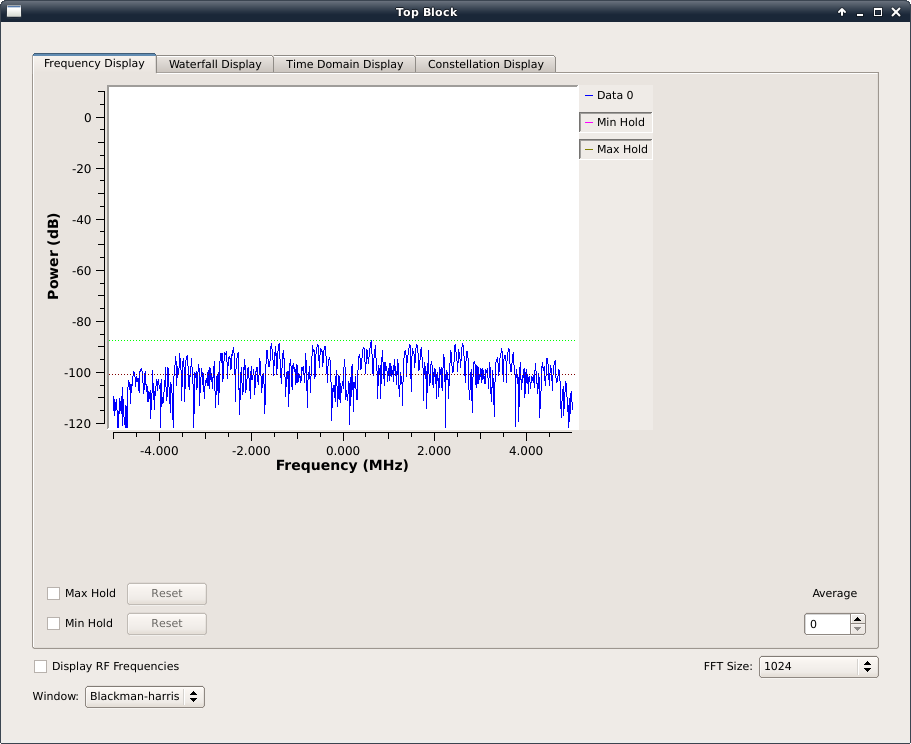
\includegraphics[width=\textwidth]{images/mon_1k_ping.png}
%	}
%	\subfloat[]{
%		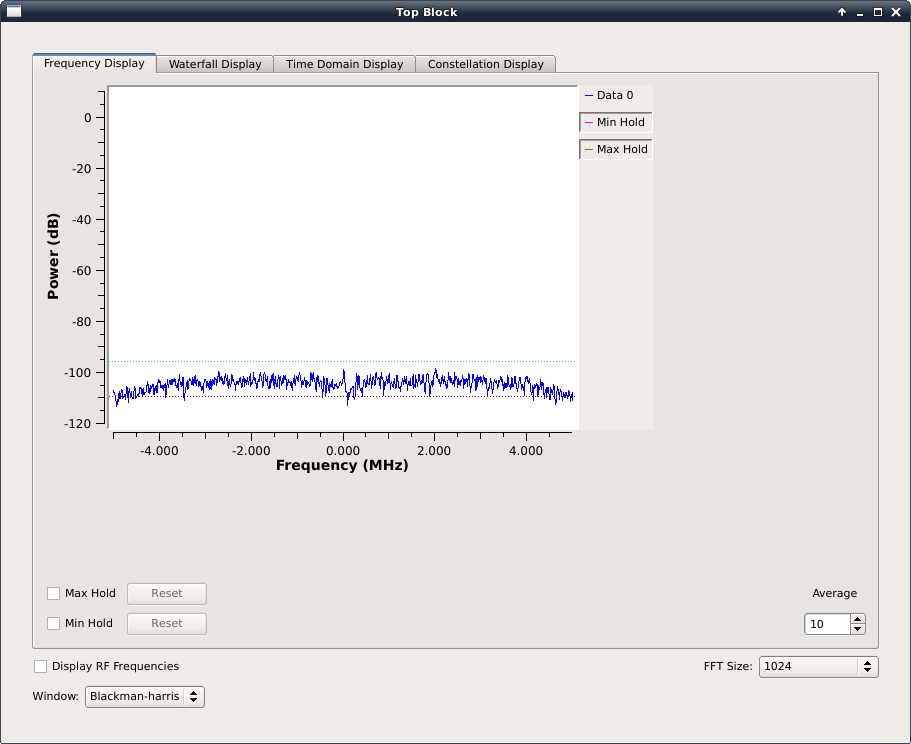
\includegraphics[width=.5\textwidth]{images/mon_nojam_ping.png}
%		
%	}
	\caption{Ping signal and jamming signal with 1kHz bandwidth. The jamming signal is hardly visible.}
	\label{1k:jam}
	\end{figure}
	

\subsection{Jamming with 100kHz bandwidth}
	After finishing the first jamming attempt, the attacking team changed the cut-off frequency of low pass filter to $100kHz$ increasing in this way the bandwidth of the jamming signal.
	\begin{hypo}
		In this second attempt, we can hypothesize that the jamming attack will be effective , as we increased the bandwidth.
	\end{hypo} 

	After starting the jamming signal (\autoref{100k:attack}), we observe that the ping command is interrupted, as the client receives messages: "Host unreachable".
	\begin{figure}
		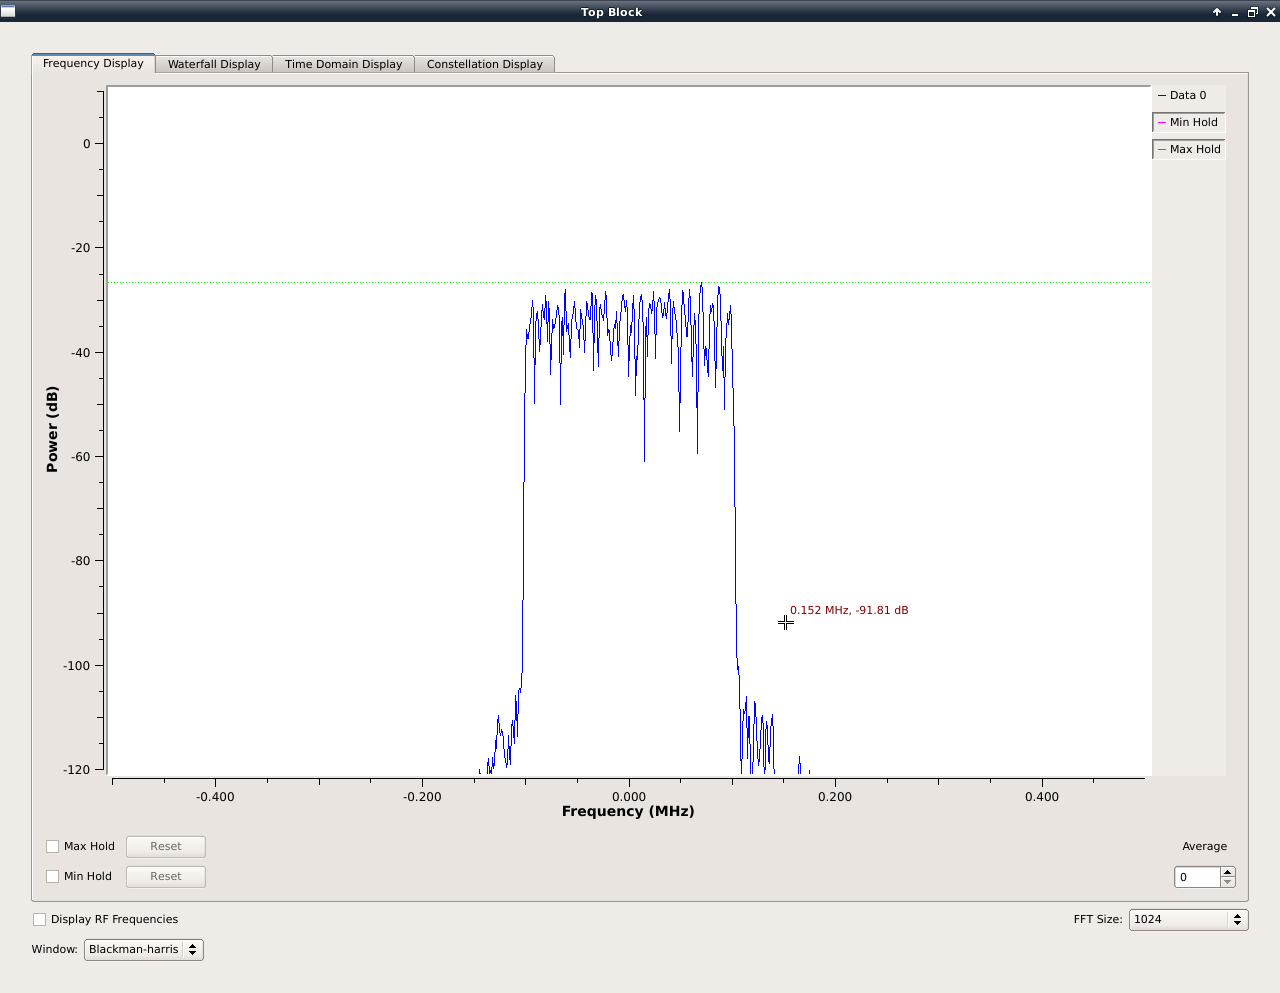
\includegraphics[width=\textwidth]{images/attack_100kHz.png}
		\caption{Jamming signal with 100kHz bandwidth observed on the \emph{Attacking device}}
		\label{100k:attack}
	\end{figure}
	One interesting point in this case is that with very limited jamming bandwidth (100 kHz), we managed to interrupt the communication in a Wi-Fi channel, that has 22 MHz bandwidth. See \autoref{100k:attack}.
	\begin{figure}
		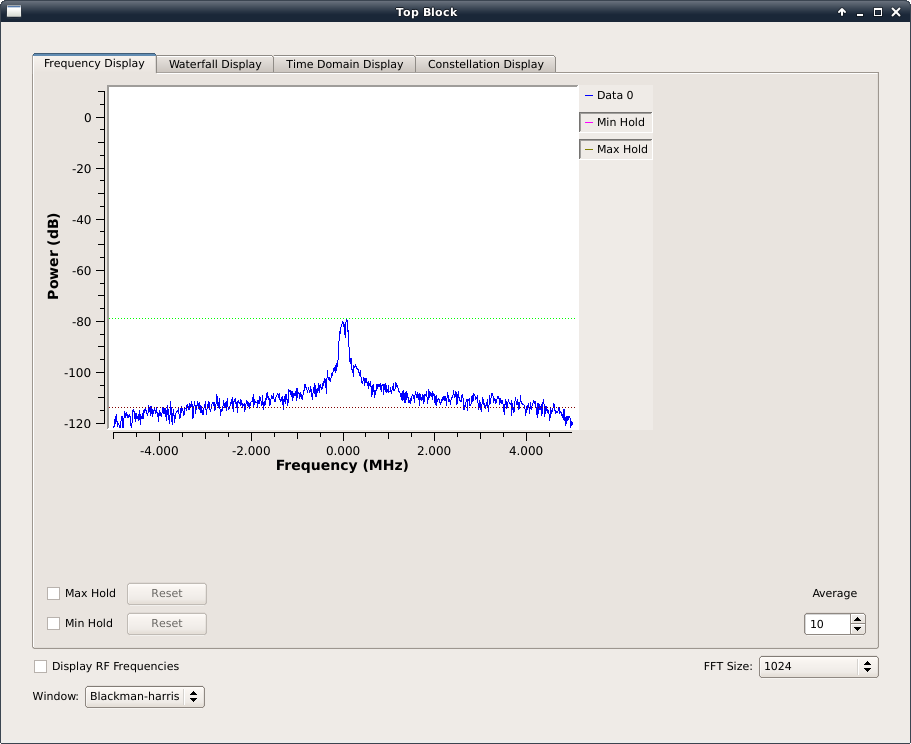
\includegraphics[width=\textwidth]{images/mon_100k.png}
		\caption{Ping and jamming signal with 100kHz bandwidth observed on the \emph{Monitoring device}. The peak in the center is the jamming signal.}
		\label{100k:attack}
	\end{figure}
	
	This outcome is due to the fact that the 802.11 b standard uses very short, 11bit, pseudorandom code length for the DSSS modulation. This means the signal is only spread a little, resulting in a narrow bandwidth and thus being more prone to jamming.
	Using longer codes could solve this. 

\subsection{Jamming with infinite bandwidth}
	In third approach we removed the low-pass filter from the jammer.
	\begin{hypo}
		Jamming on all frequencies will stop all ping transmissions, not only our group's, but the other groups' as well.
	\end{hypo}
	
	This turned out to be partly true.
	Our transmission was in fact stopped, but not the other's.
	We assume this due to the distance to the other's receivers.
	Notice that the peak power of the jammer was still set to the same value and that the power of the signal should not have gotten spread over more frequencies, if the radio could have provided enough power. 
	But apparently this was not the case and we assume that the devices maximum power got spread over a large frequency range.
	See \autoref{all:freq}.
	
	\begin{figure}
		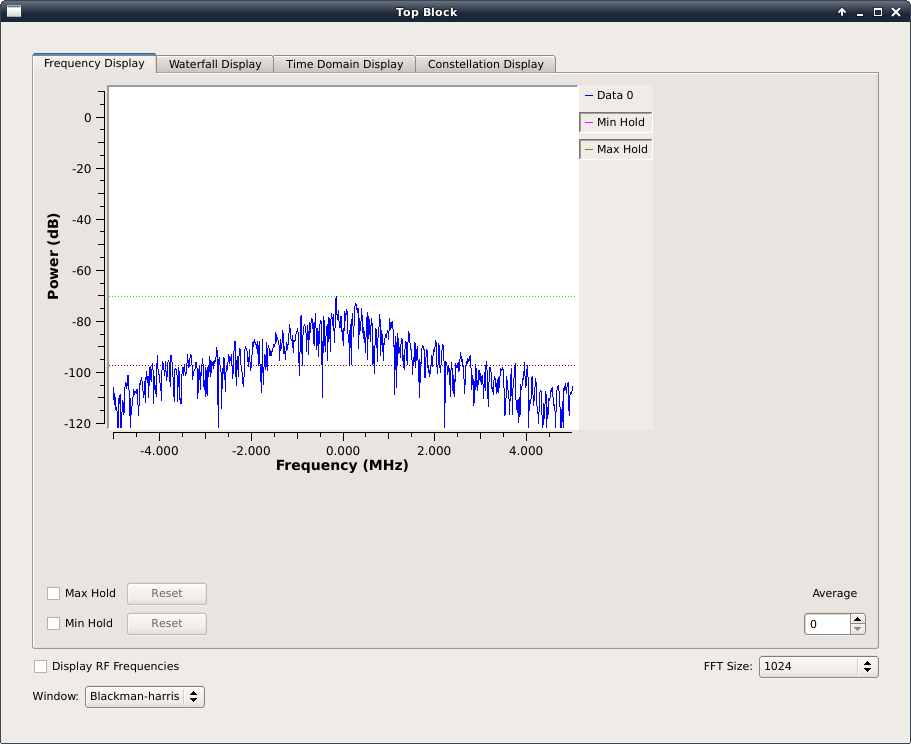
\includegraphics[width=\textwidth]{images/mon_jamallfrequ_ping.png}
		\caption{Jamming and ping signal when no filter is applied to the jamming signal.}
		\label{all:freq}
	\end{figure}
	
\section{Analysis}
After completing the lab exercise about Jamming Resistant Communication, we can summarize the following statements:
\begin{itemize}
\item Without jamming we could observe a pattern similar to a \texttt{sinc} function in the frequency domain.
\item We observed that a jamming signal of narrow bandwidth is able to interrupt a DSSS modulated communication if short chip-codes are used. 
\item The Jamming attack can be sometimes ineffective and this is due to its narrow bandwidth, its weak transmission power, or its long distance from its target. 

\end{itemize}

\bibliographystyle{plain}
\bibliography{bibliography}
\end{document}